\documentclass[11pt]{article}
\newcommand{\Comment}[1]{}
\newcommand{\todo}[1]{{\color{red}\bfseries [[#1]]}}
\newcommand{\kmp}{KMP\xspace}
\newcommand{\wu}{Wu\-Manber\xspace}
\newcommand{\pmt}{PMT\xspace}
\newcommand{\lz}{LZ78\xspace}
\newcommand{\lsa}{Linear Suffix Array\xspace}
\newcommand{\sa}{Suffix Array\xspace}
\newcommand{\ipmt}{{\it ipmt}\xspace}
\newcommand{\gzip}{gzip\xspace}
\newcommand{\rqone}{Como a nossa implementa\c{c}\~ao do \lz se compara ao \gzip?}
\newcommand{\rqtwo}{Como a etapa de busca de padr\~ao do \ipmt se compara ao grep?}
\newcommand{\rqthree}{Como a nossa implementa\c{c}\~ao do \ipmt se compara ao
codesearch?}
\newcommand{\lst}{Linear Suffix Tree\xspace}

\usepackage{xspace}
\usepackage[utf8]{inputenc}
\usepackage[portuguese]{babel}
\usepackage{relsize}
\usepackage{longtable}
\usepackage{booktabs}
\usepackage{array}
\usepackage{mathtools}
\usepackage{url}
\urlstyle{same}  % (sf also works, for something more subtle than tt)
\usepackage{color}
\usepackage{graphicx}
%% Colors
\definecolor{darkred}{rgb}{0.5,0,0}
\definecolor{darkgreen}{rgb}{0,0.5,0}
\definecolor{darkblue}{rgb}{0,0,0.5}
\usepackage[bookmarks=false]{hyperref}
\hypersetup{ colorlinks,
  linkcolor=darkblue,
  filecolor=darkgreen,
  urlcolor=darkred,
  citecolor=darkblue }

\begin{document}

\begin{center}
UNIVERSIDADE FEDERAL DE PERNAMBUCO – UFPE\\
CENTRO DE INFORMÁTICA – CIn\\[10\baselineskip]
\end{center}

\begin{center}
Relatório do projeto da disciplina:\\
Processamento de Cadeias de Caracteres
(2015.2)\\[10\baselineskip]
\end{center}
Equipe:\\
João Guilherme Farias Duda\\
Paulo de Barros e Silva Filho\\
Raul Maia Falcão\\[8\baselineskip]


\begin{center}
Recife, 3 de Janeiro de 2016
\end{center}

\cleardoublepage

\tableofcontents

\cleardoublepage
\section{Introdução}

Este documento é sobre a ferramenta \ipmt. Essa ferramenta é capaz de
pré-processar um arquivo de texto, gerando um índice. Sucessivas buscas podem
ser feitas através desse índice, sem a necessidade de percorrer o texto
novamente.


\ipmt primeiro gera um índice para o texto usando o algoritmo LSA (Linear Suffix
Array), depois esse índice é comprimido em um arquivo juntamente com o texto
usando o algorítmo \lz. Para realizar buscas, primeiramente o arquivo é
descomprimido usando o \lz-decode e depois o casamento de padrões é realizada
de acordo com o LSA.


Os integrantes da equipe foram responsáveis pelas seguintes tarefas:
\begin{itemize}
\item João: 

\item Paulo: Implementação do algorítmo \lz e da interface de comunicação entre os algoritmos.

\item Raul: Implementação das estruturas de indexação \lsa (LSA) e Linear Suffix Tree (ST).

\end{itemize}



\section{REQUISITOS}


\section{Descrição de uso da ferramenta \ipmt}

O projeto contém um arquivo Makefile. Após a execução do comando make, o
executável \ipmt será gerado no diretório bin. A ferramenta \ipmt possui 4 modos
de execução:

\begin{itemize}

\item Modo de indexação - \ipmt index file.txt

    O comando acima irá criar o arquivo file.idx, que contém o conteúdo de
    file.txt e que possibilita a realização de buscas.

\item Modo de busca - \ipmt search -c herself file.idx

    O comando acima irá listar a quantidade de ocorrência do padrão "herself"
    encontradas no arquivo indexado file.idx. O argumento -c é opcional, caso
    não informado todas as linhas contendo ocorrências serão impressas.

\item Modo de compressão - \ipmt compress file.txt

    O comando acima irá comprimir o arquivo file.txt em um arquivo file.comp.

\item Modo de descompressão - \ipmt decompress file.comp

    O comando acima irá descomprimir o arquivo file.comp em um arquivo
    file.comp.decomp.

\end{itemize}


\section{Implementação}
Todos os algoritmos foram implemetados em C++ por questões de eficiência. A
implementação em Python feita em sala de aula foi usada como uma base inicial.

\subsection{Descrição dos algoritmos implementados}

\subsubsection{\lsa}
O algoritmo de indexação  implementado teve como
base~\cite{KarkkainenS03} para a construção em
tempo linear de um array de sufixos. Em suma, o array de sufixos é um array de
inteiros que armazena a permutação de n índices ordenados lexicograficamente,
onde n é o tamanho do texto. Uma vez construído o array de sufixos, a
complexidade da busca passa a ser linear com relação ao tamanho do padrão.

\subsubsection{\lst}
O algoritmo de indexação implementado teve como
base ~\cite{UkkonenST} para a construção em tempo linear
de uma árvore de sufixos. A estrutura implementada representa
todos os sufixos de uma cadeia. A implementação contém alguns truques
para que a construção seja feita em tempo linear. Um desses truque é adicionar aos
nós suffix links, também chamados como transições de falha ou fronteiras. Devido 
ao alto consumo de memória ao gerar a árvore de sufixo, resolvemos deixar a feature
de melhorar o gerenciamento de memória para o futuro. Por consequência não foi gerado os índices dos sufixos, mas existe a opção de busca exata retornando o número de ocorrências de um dado padrão. Segundo ~\cite{BogdanCraig} se o núcleo da implementação for orientada a objeto, a árvore de sufixo apresenta efeitos indesejáveis
de memória fragmentada.

\subsubsection{\lz}

O algoritmo de compressão \lz teve como base a implementação vista em sala de
aula e descrita em~\cite{Storer:1987:DCM:42791}. O \lz utiliza um dicionário
dinâmico explícito, onde a referência compreende um par composto pelo índice no
dicionário e o caracter de mismatch.

Durante a compressão (\lz-encode), o dicionário é criado dinâmicamente a cada
mismatch. Junto com o dicionário, também é criado um código que representa a
string que está sendo comprimida. O \lz-encode é linear de acordo
com o tamanho da string que está sendo comprimida.

O processo de descompressão (\lz-decode) recebe somente o código gerado durante
a compressão, e é capaz de gerar o dicionário dinamicamente, bem como a string
original que foi comprimida. O \lz-decode é linear de acordo com o tamanho do
código recebido na entrada.


\subsection{Detalhes de implementação}
Abaixo descrevemos algumas decisões e peculiaridades de cada algoritmo.

\subsubsection{\lsa}

Na construção do \lsa há uma etapa de criação de dois arrays de sufixos, S1 e S2.
Seja index a posição de um caracter em um texto:  A função buildS1andS2 constrói
o array de sufixo S1 que contém sufixos tal que index \% 3 = 0 e também constrói
o array de sufixo S2 que contém sufixos tal que index \% 3 != 0. Após a
construção de S1 e S2, estes são ordenados através de uma implementação do Radix
Sort com o objetivo de otimizar essa etapa. Como o Radix Sort não faz
comparações entre valores, nesse contexto, o seu desempenho é superior a um
algoritmo de ordenação por comparação. A ordenação de S1 e S2 foi necessária
para a etapa de merge (S1  U  S2 = SA)  de tal forma que o custo do merge é
realizado em tempo linear. Após o merge, obtemos os índices devidamente
ordenados.

\subsubsection{\lst}
Inicialmente na construção do \lst foi necessário criar um nó auxiliar ($\perp$) o qual possue transições de todas as letras do alfabeto para o nó inicial (root) que corresponde a uma cadeia vazia ($\varepsilon$). Após essa etapa, uma construção on-line é feita adicionando caracter por caracter a árvore através das funções $update$ e $canonize$. A função update transforma a árvore na iteração anterior em uma árvore na iteração corrente inserindo transições do caracter corrente a ser adicionado. A função $update$ utiliza a função $canonize$ e a função $test{\_}and{\_}split$ que testa se há ou não referência a um nó terminador. Ao final da função $update$ é retornado a referência do par do nó terminador. Após adicionar todos os caracteres a árvore de sufixo está devidamente montada e pronta para realizar buscas de padrões exatos.

\subsubsection{\lz}
O dicionário dinâmico possui uma estrutura de Trie: Cada nó mapeia um índice a
somente um char, e possui nós descendentes de forma que o nó original e cada um
de seus descendes forma uma sequência diferente de caracteres encontrada no
texto.

Usamos como alfabeto do código de saída o sistema binário. Como cada elemento do
código de saída tem somente um bit, usamos como estrutura de dados para guardar
o código um vector de
bool\footnote{\url{http://en.cppreference.com/w/cpp/container/vector_bool}}.
Optamos por essa estrutura de dados pois ela possui uma otimização de espaço:
Um bool em C++ ocupa 8 bits (1 byte) de espaço na memória, porém um vector de
bool usa somente 1 bit para cada elemento.

Outra peculiaridade desse algorítmo é que pode ocorrer do arquivo descomprimido
conter algum "lixo" no último byte. Isso acontece porque a escrita em arquivo só
pode ser feita de byte em byte, porém o código gerado pelo \lz-encode é uma
sequência de bits. Caso o número de bits não seja um múltiplo de 8, o último
byte precisa ser preenchido com uma sequência de 0s, o que pode alterar o último
byte na hora da descompressão. Isso poderia ser contornado com alguma flag no
início do arquivo comprimido, informando quantos bits devem ser descartados do
último byte. Deixamos isso como trabalho futuro.

\subsection{Descrição do formato .idx}

A ferramenta \ipmt gera e lê arquivos no formato .idx. Esse arquivo é gerado da
seguinte forma para um arquivo de entrada file.txt:

\begin{enumerate}

\item Primeiramente é gerado o \lsa a partir do conteúdo de file.txt.
\item Após isso, conta-se o número de linhas de file.txt.
\item É criado um novo arquivo com o seguinte contéudo:
\begin{verbatim}
            [Número de linhas contidas em file.txt]
            [Conteúdo de file.txt]
            [Elementos do LSA separados por um espaço]

(Note que quebras de linha separam os elementos acima.)
\end{verbatim}
\item Esse novo arquivo é então comprimido usando o \lz, gerando o arquivo file.idx.

\end{enumerate}

Na hora de ler o arquivo .idx, primeiro é realizada a descompressão. Através do
resultado, a ferramenta sabe que a primeira linha contém o número de linhas do
texto. Logo, as linhas seguintes são referentes ao LSA, que é utilizado pela
busca.


\section{Experimentos}
Comparamos nossas implementações com o
\gzip\footnote{\url{http://www.gzip.org/}},
grep\footnote{\url{https://www.gnu.org/software/grep/}} e com o
codesearch\footnote{\url{https://github.com/google/codesearch}}.
Realizamos experimentos para responder às seguintes perguntas:
\begin{enumerate}
\item \rqone
\item \rqtwo
\item \rqthree
\end{enumerate}

Foram implementados scripts em BASH para controlar os experimentos e fazer
medições, gerando arquivos .raw de saída contendo resultados. Foram também
implementados scripts em R que desenham gráficos de acordo com os arquivos .raw
gerados pelos scripts BASH.


Todos os experimentos foram realizados em uma máquina com processador Intel Core
i5 2.6Ghz e 8Gb de RAM. Cada medição de tempo nos experimentos foi realizada 10
vezes, e somente a média foi considerada e reportada nos resultados.
Todos os scripts e resultados estão disponíveis no diretório {\it experiments}.

\subsection{\rqone}
Nós comparamos a nossa implementação do \lz com o \gzip em dois aspectos: Tempo
e taxa de compressão.
Para realizar essa comparação, nós dividimos um arquivo\footnote{
\url{http://pizzachili.dcc.uchile.cl/texts/nlang/english.1024MB.gz}}
que contém 1GB de texto em inglês em arquivos de
tamanhos distintos: 100KB, 200KB, 300KB, 700KB, 1MB, 2MB, 3MB, 5MB, 50MB, 100MB,
200MB, 300MB e 500MB. Cada arquivo desse contém os primeiros n bytes do
arquivo original, onde n é o tamanho do arquivo.

\subsubsection{Tempo}

Abaixo está um gráfico que relaciona o tempo que leva para comprimir um arquivo
com o tamanho dele, para ambos o nosso \lz e o \gzip.
\\
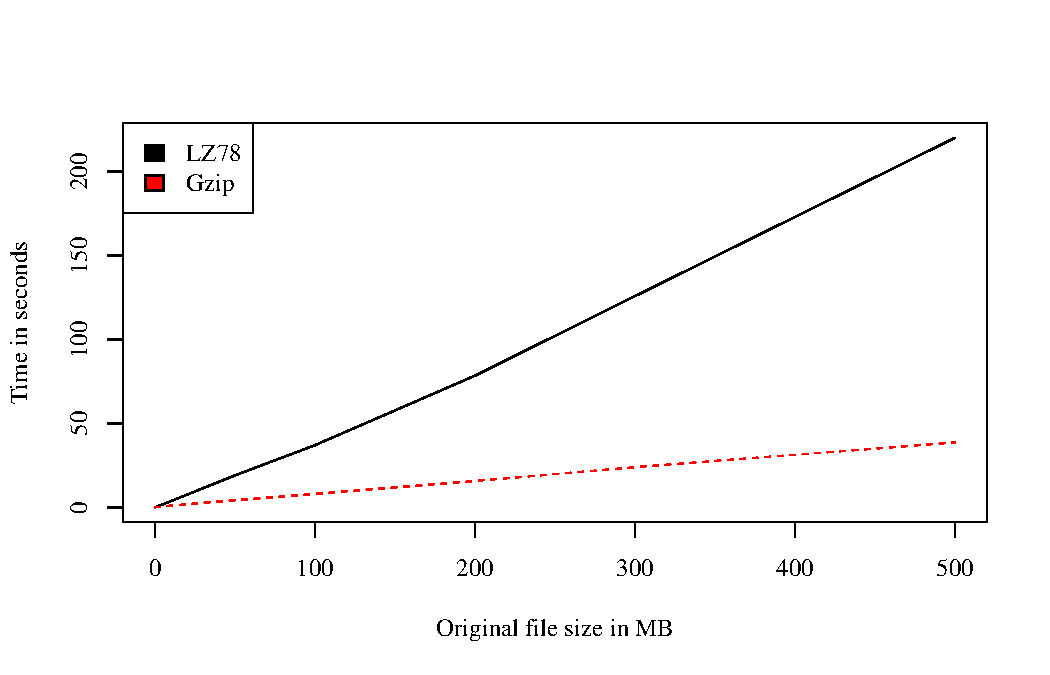
\includegraphics[scale=0.74]{../experiments/R/pdf/time_comp}
\\

Ambas as funções são (ou se aproximam muito de) retas, o que comprova que a
nossa implementação do \lz, bem como o \gzip, comprimem em tempo linear de
acordo com o tamanho do arquivo. Porém, a constante que multiplica a função do
\gzip é bem menor do que a nossa. Isso acontece porque o \gzip está em
desenvolvimento a mais de 23 anos, onde experts estão sempre otimizando o
algoritmo, fazendo com que essa constante da função linear seja cada vez menor.


Os arquivos comprimidos acima foram descomprimidos com ambas as ferramentas \lz
e \gzip. Abaixo está um gráfico que relaciona o tempo que leva para descomprimir
um arquivo e o tamanho dele.
\\
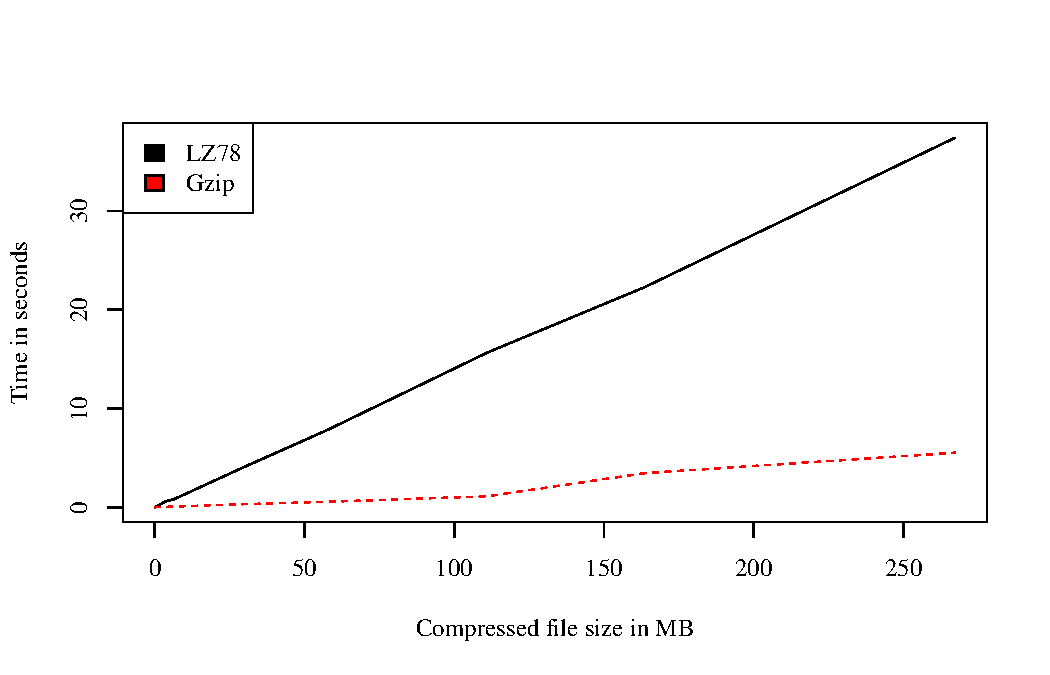
\includegraphics[scale=0.74]{../experiments/R/pdf/time_decomp}
\\

Obtivemos novamente um resultado consistente com o anterior: ambos possuem
complexidade linear, porém a constante da descompressão do \gzip é muito
superior à da nossa implementação. Isso ficou ainda mais acentuado na
descompressão do que na compressão.

\subsubsection{Taxa de compressão}

Abaixo está um gráfico que relaciona a taxa de compressão de um arquivo com o
tamanho original dele, para ambos o nosso \lz e o \gzip.
\\
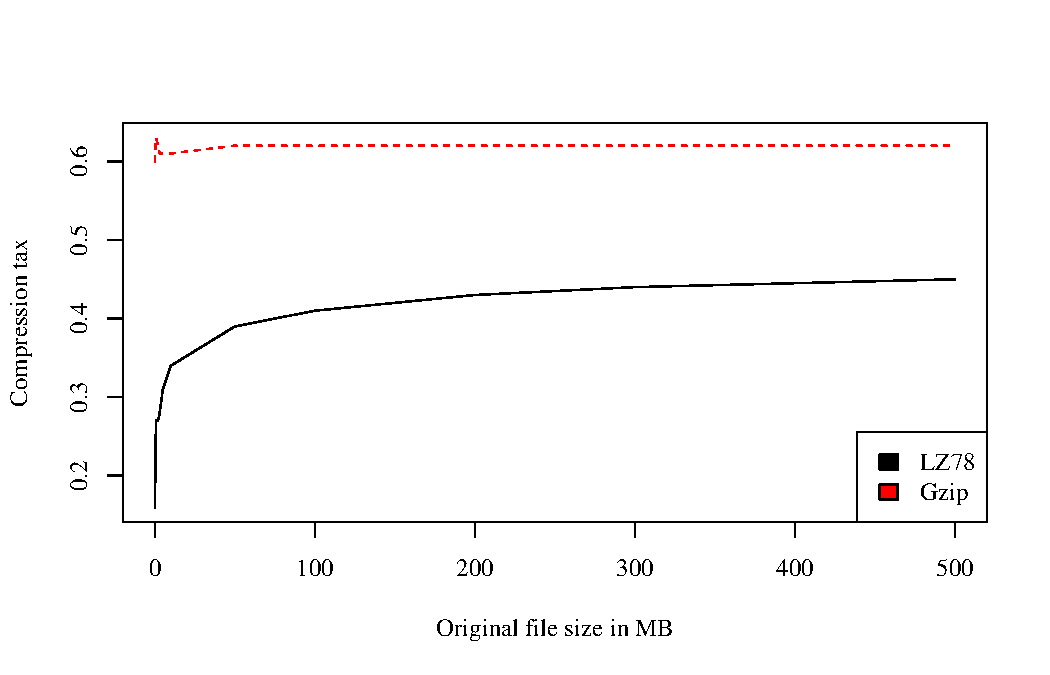
\includegraphics[scale=0.74]{../experiments/R/pdf/comp_tax}
\\

Novamente, os resultados se assemelham quando analisados separadamente:
Ambos possuem uma variação inicial (apesar do \gzip ter uma bem menor) e se
estabilizam para arquivos maiores. Porém, o \gzip se estabiliza com uma taxa de
compressão próxima de 60\%, enquanto que o nosso \lz se estabiliza com uma taxa
próxima de 42\%. Recorremos novamente ao argumento de que o \gzip está em
desenvolvimento a muito mais tempo e por isso possui mais otimizações.

\subsection{\rqtwo}
Para responder à essa pergunta nós utilizamos a ferramenta \ipmt para criar um
índice de um arquivo de texto. Após isso comparamos o tempo de realizar buscas
de diversos padrões utilizando \ipmt no arquivo indexado e comparando com o
tempo para pesquisar os padrões utilizando grep no texto original.

Nós consideramos somente o arquivo de 50MB pelo seguinte motivo: O arquivo .idx
gerado pela ferramenta \ipmt possui ambos o texto original e o índice
comprimidos. Acontece que o array do nosso LSA tem, em média, quase 10 vezes o
tamanho do arquivo original. Ou seja, indexar e comprimir um arquivo de 50MB
acaba se tornando uma tarefa de comprimir um arquivo de aproximadamente 500MB,
que dura pouco mais de 4 minutos. Nesse caso, nossa compressão criou um arquivo
.idx de 341MB, onde as buscas serão realizadas. Indexar e comprimir arquivos
maiores do que 50MB é uma tarefa custosa para nossas implementações.



\subsection{\rqthree}

\todo{add text}



\Urlmuskip=0mu plus 1mu\relax
\bibliographystyle{abbrv}
\bibliography{tmp}

\end{document}
